% Or call it Research results?

\chapter{Experiments and Results}
\label{chap:experiments-and-results}
This chapter presents the experiments and results that have been conducted. The experiments are grouped by research question. First, experiment \textbf{E1} takes on research question 1 regarding automatic smart contract code synthesis. It compares the performance of pre-trained transformer-based language models on the verified smart contract dataset. Experiment \textbf{E2} focuses on the security of smart contract code generation, tackling research question 2. It compares the security of a fine-tuned model utilizing security conditioning purposed in \cref{sec:security-conditioning}. This section presents three sub-experiments:
\begin{enumerate}[label=\textbf{E2.\arabic*.}, leftmargin=1.5cm]
    \item Compares security performance based on providing entire class context from audited verified smart contract dataset.
    \item Compares security performance based on using only comments as input context from audited verified smart contract dataset.
    \item Compares security performance based on testing a custom vulnerability-inclined dataset.
\end{enumerate}

The last experiment \textbf{E3} takes on research question 3 regarding how to best formulate the input for automatic smart contract code synthesis.

\section{E1 - Automatic Smart Contract Code Synthesis}
\label{sec:e1-automatic-smart-contract-code-synthesis}

\subsubsection{Goal}
\subsubsection{Method and Data}
\subsubsection{Results and Discussion}

\begin{figure}[htp]
    \centering
    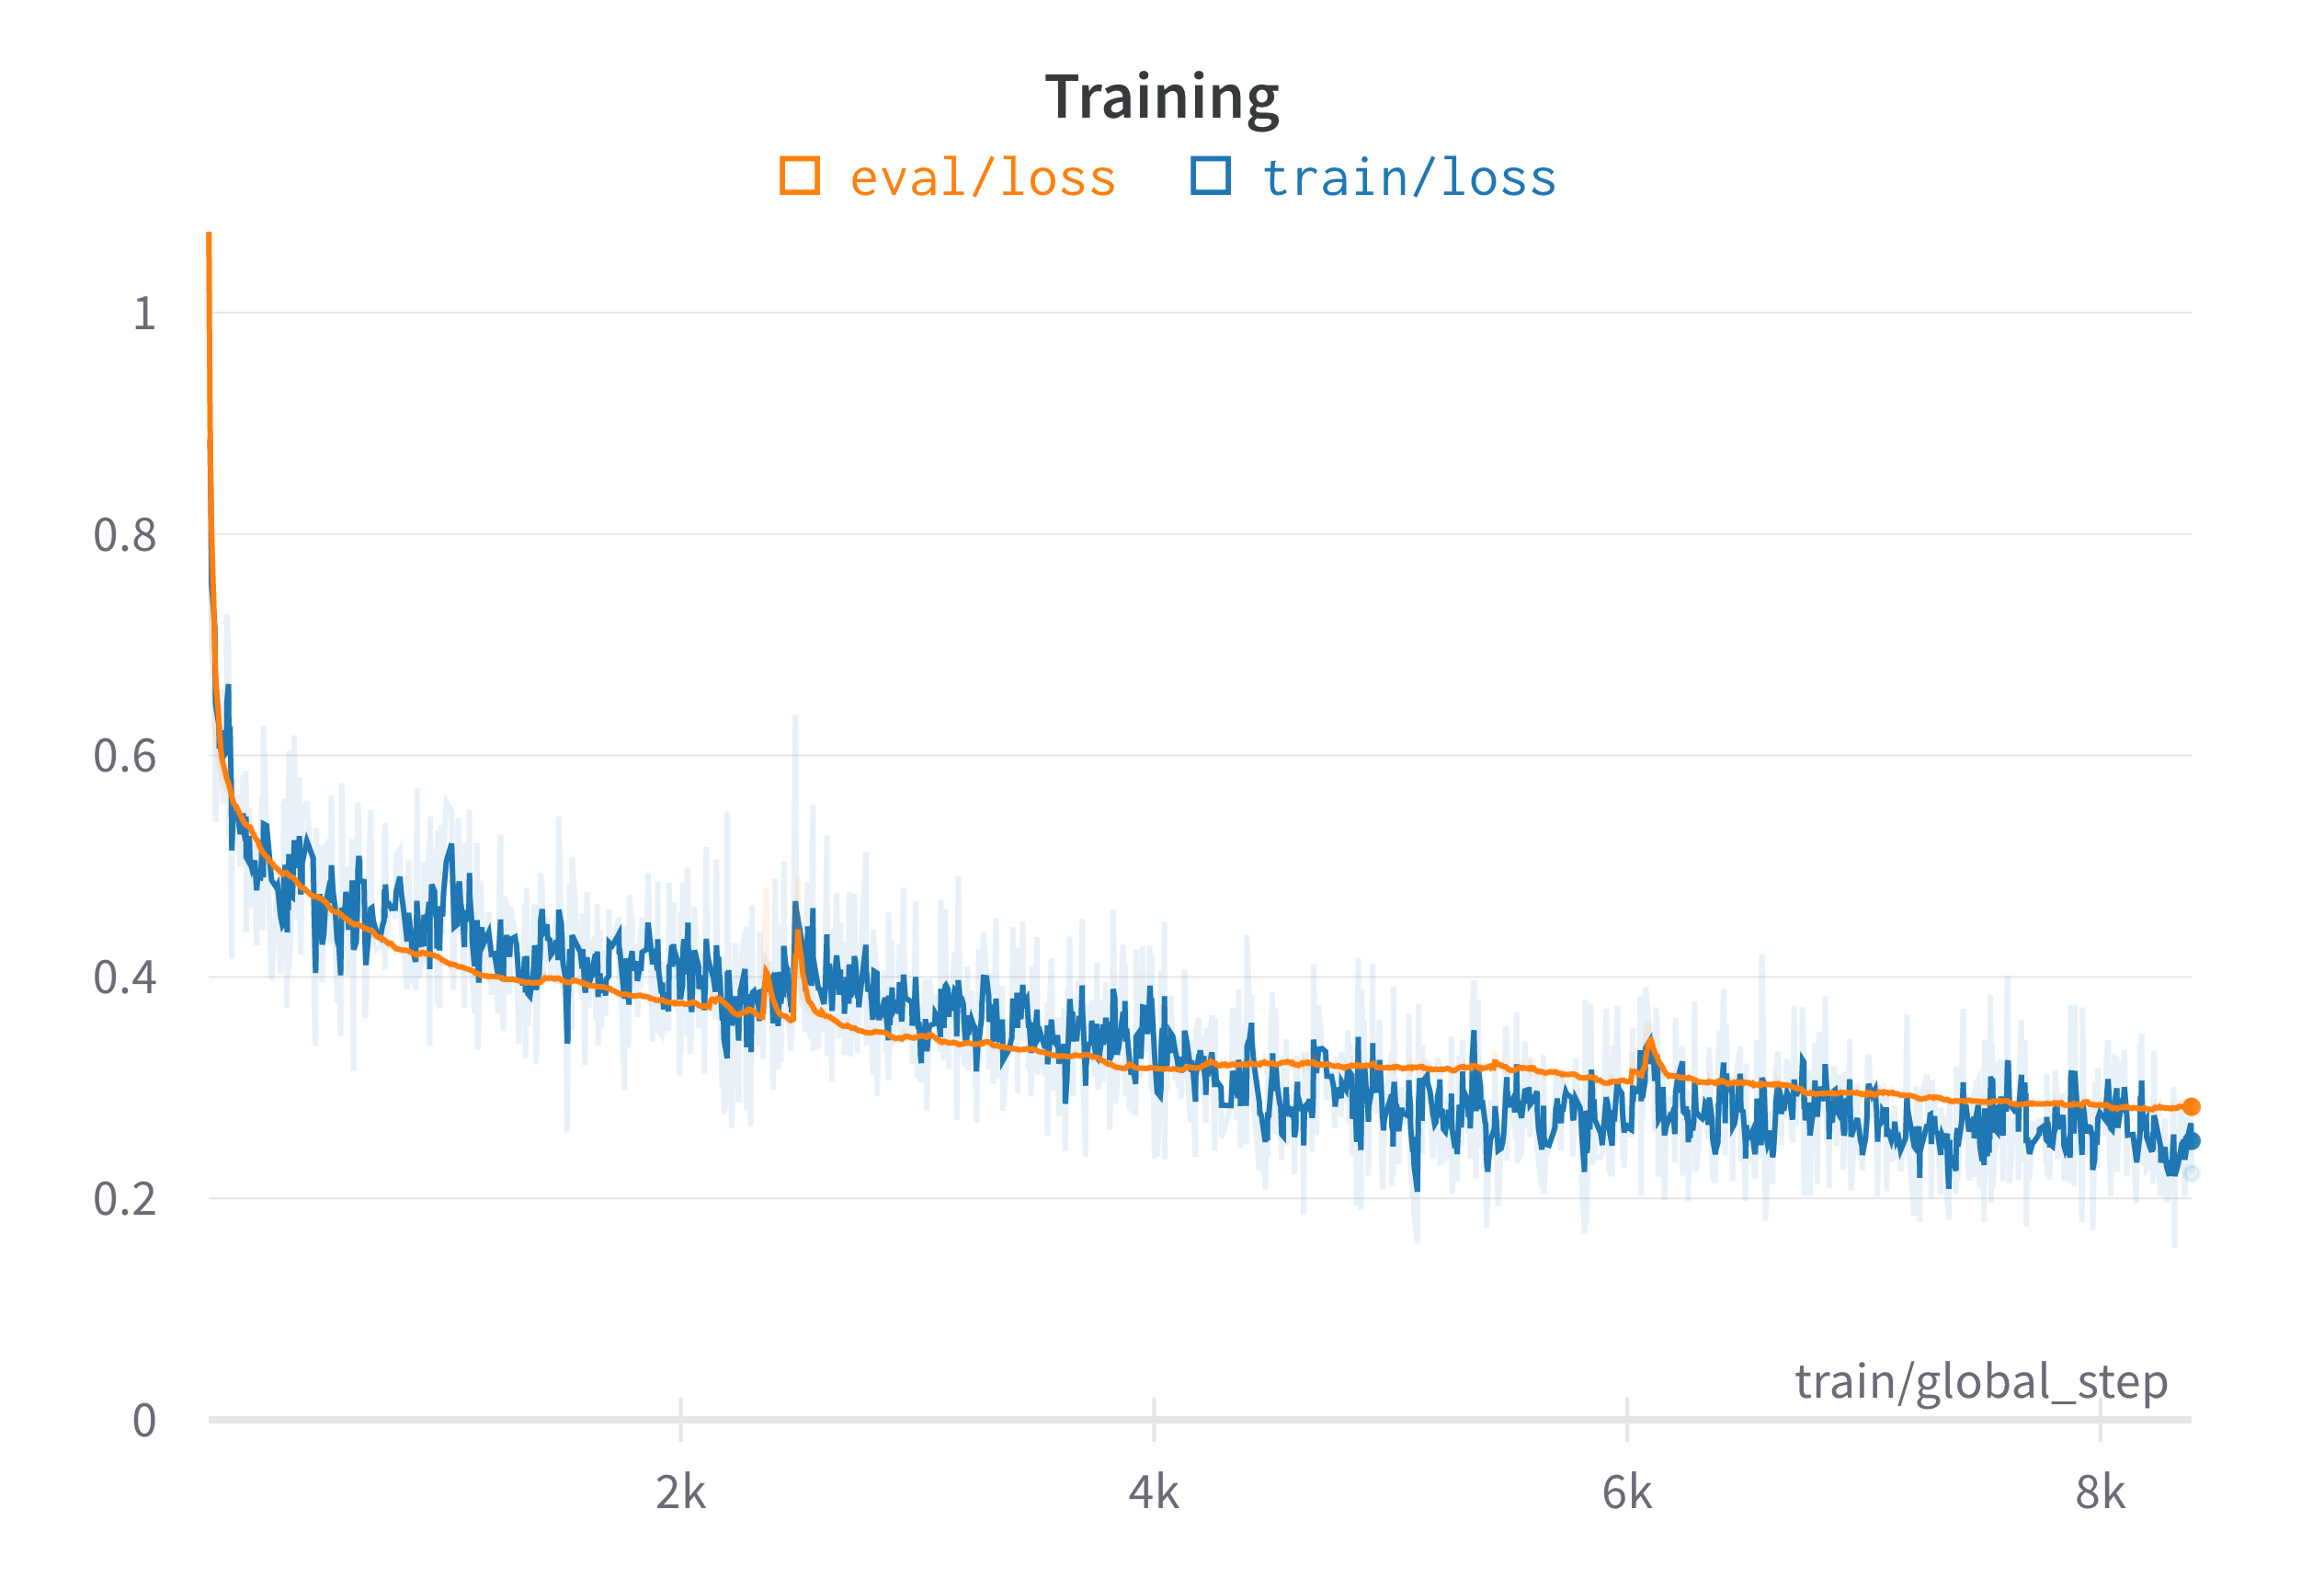
\includegraphics[width=\textwidth]{figures/wandb-train-loss-gpt-j-smart-contract.png}
    \caption{Training and evaluation loss during model training.}
\end{figure}

\begin{figure}[htp]
    \centering
    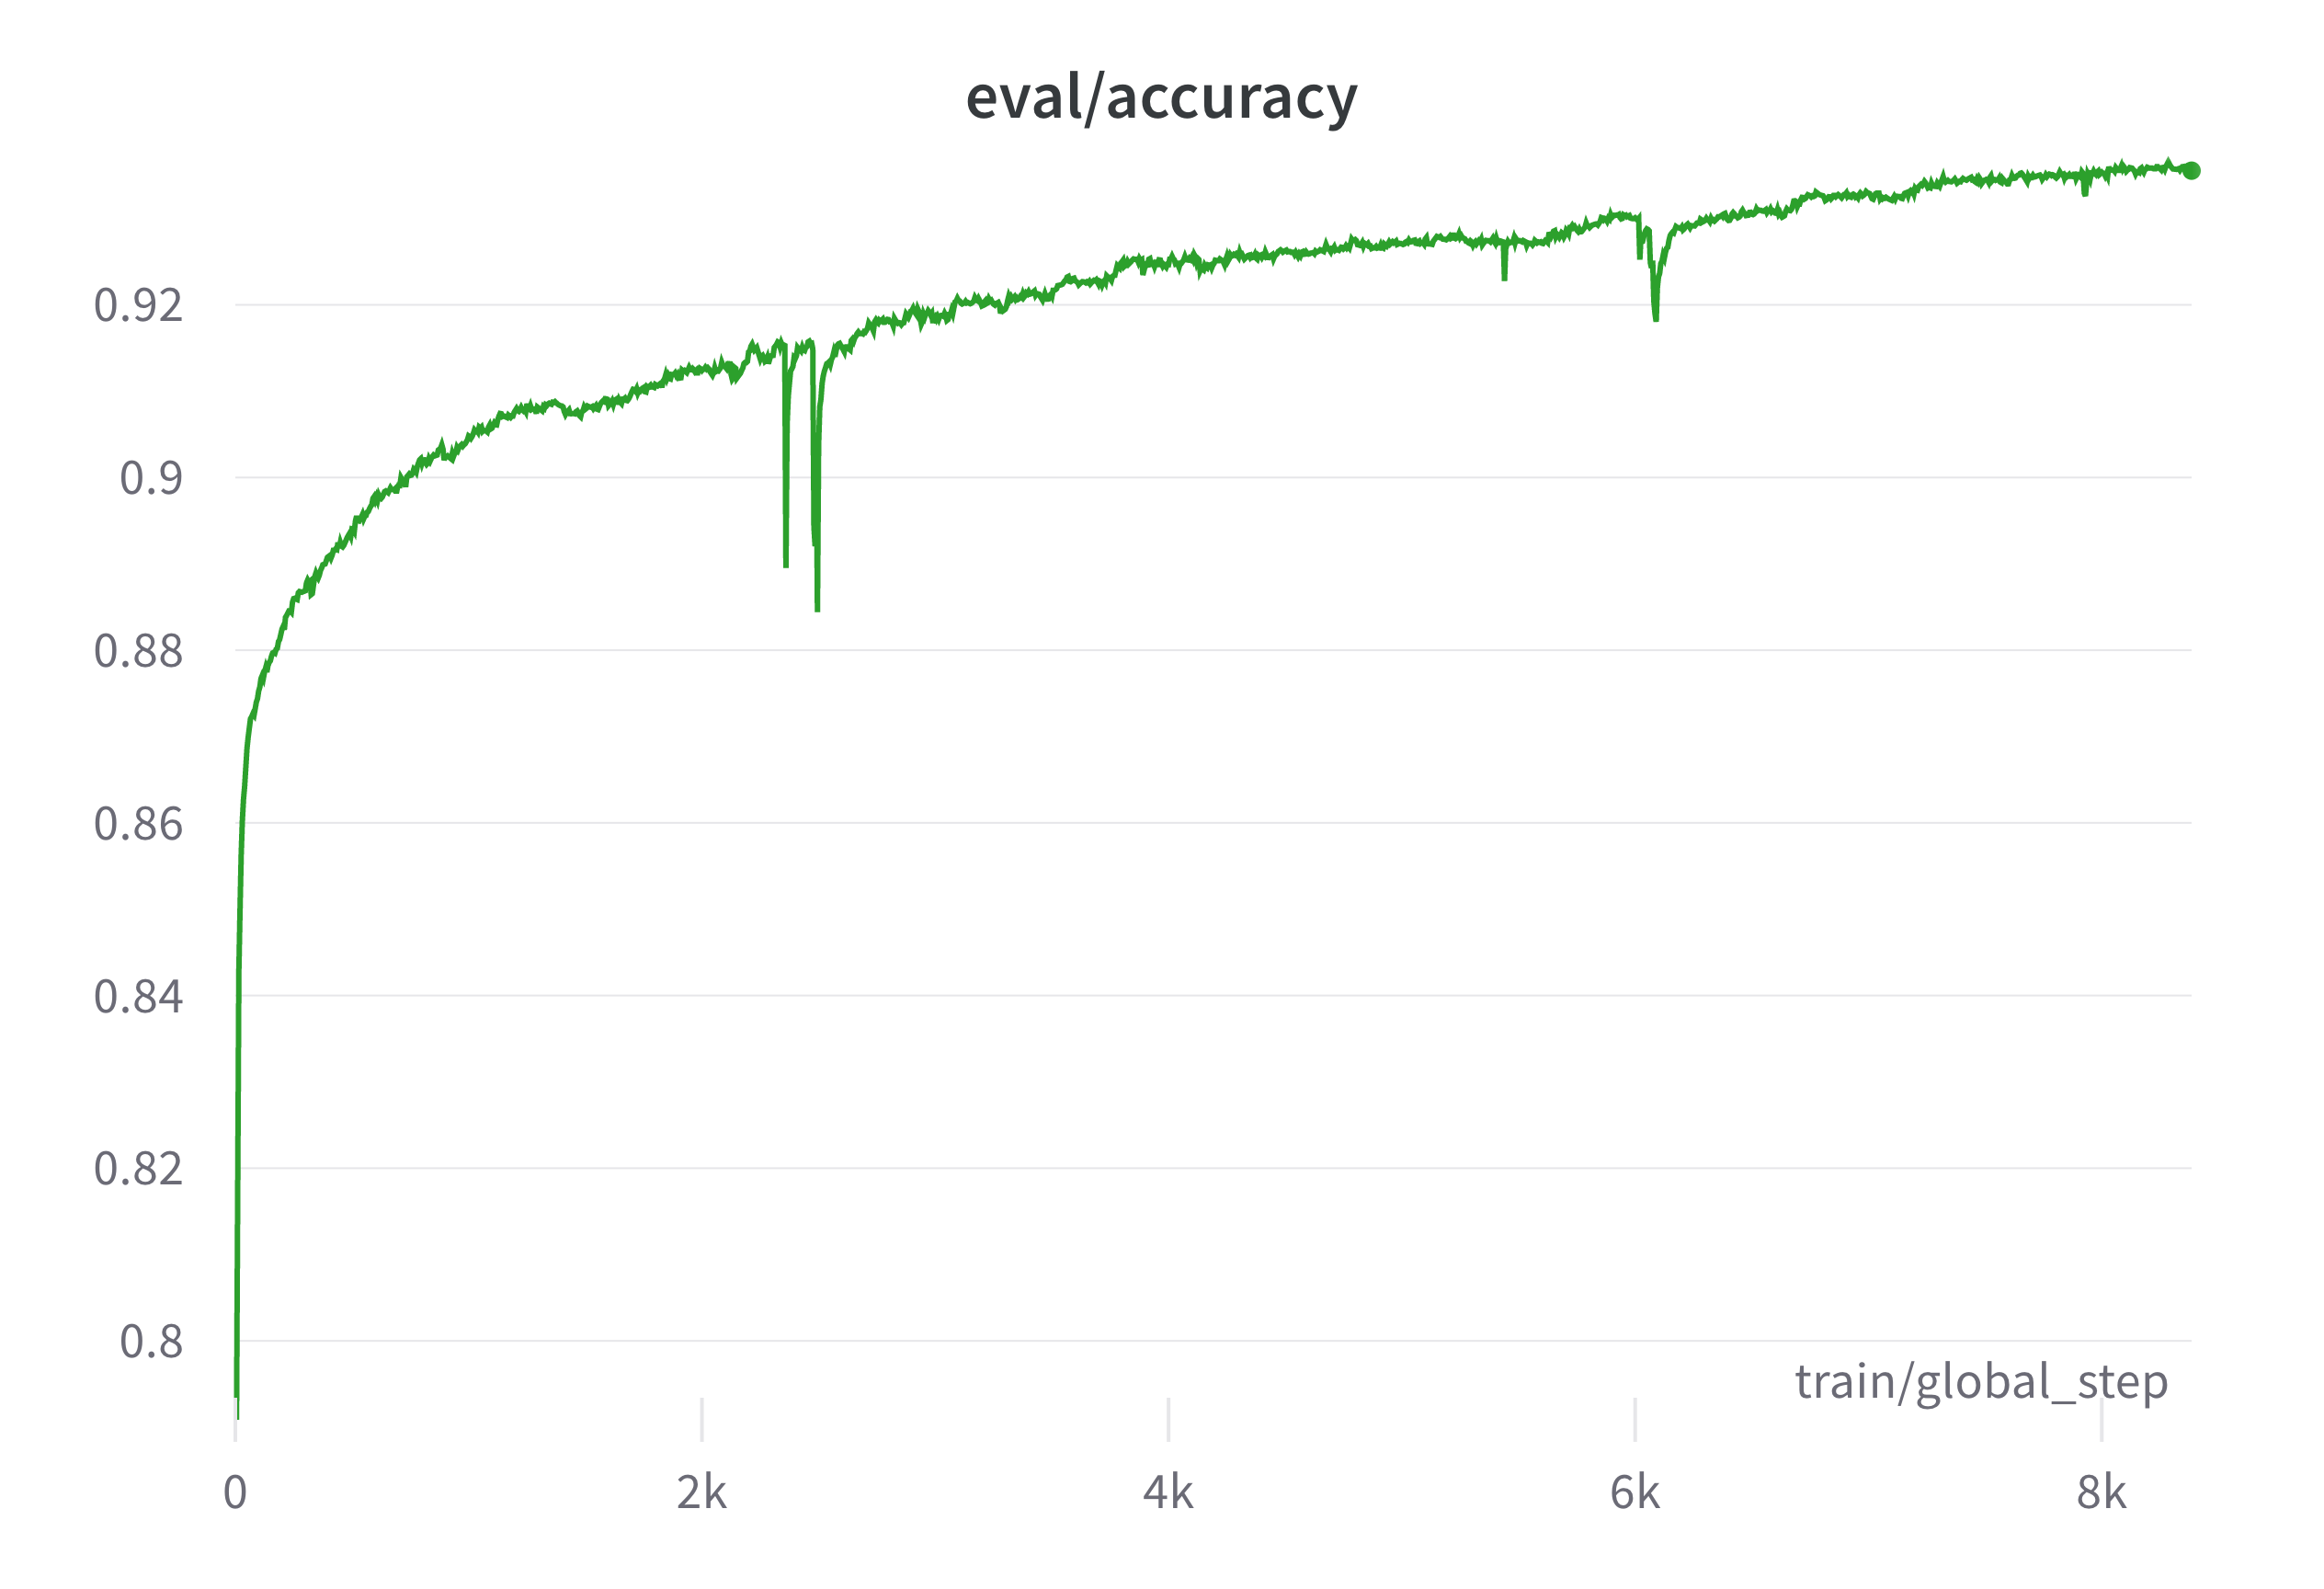
\includegraphics[width=\textwidth]{figures/wandb-train-eval-gpt-j-smart-contract.png}
    \caption{Evaluation accuracy during model training.}
\end{figure}


\section{E2 - Security Conditioning}
\label{sec:e2-security-conditioning}
This section presents the results and discussion of the sub-experiments of experiment \textbf{E2}. Experiment \textbf{E2} focuses on the security of smart contract code generation, tackling research question 2. It compares the security of a fine-tuned model with and without utilizing security conditioning purposed in \cref{sec:security-conditioning}. The following three sub-experiments are all based on the same fine-tuned models, but uses different evaluation method.

\subsubsection{Goal}
\subsubsection{Method and Data}
\subsubsection{Results and Discussion}


\subsection{E2.1 - Complete Class Context}
\label{sec:e2.1-complete-class-context}

\subsubsection{Goal}
\subsubsection{Method and Data}
\subsubsection{Results and Discussion}


\subsection{E2.2 - Comment Context}
\label{sec:e2.2-comment-context}

\subsubsection{Goal}
\subsubsection{Method and Data}
\subsubsection{Results and Discussion}

\subsection{E2.3 - Inclined Vulnerabilities}
\label{sec:e2.3-inclined-vulnerabilities}

\subsubsection{Goal}
\subsubsection{Method and Data}
\subsubsection{Results and Discussion}

\section{E3 - Formulation of Inputs}
\label{sec:e3-formulation-of-inputs}

\subsubsection{Goal}
\subsubsection{Method and Data}
\subsubsection{Results and Discussion}



\todo{Move relevant stuff below to method chapter (experiment plan)}

\todo{Move to datasets?)}
\subsection{InclinedVulnerabilities}
Custom dataset containing multiple hand written INCOMPLETE contracts that MAY produce vulnerabilities.


\section{Baselines}
\subsection{InclinedVulnerabilities}

\section{Evaluation metrics}
\todo{Rewrite}
Accuracy could measure correctness of the exact match, failing, however, to capture the proximity when a completion suggestion partially matches the target sequence, which could still be a valid completion suggestion.

\todo{Rewrite}
The ROUGE score is the metric commonly used to evaluate machine translation models. Its ROUGE-L variant is based on the Longest Common Subsequence (LCS) statistics. LCS takes into account structure similarity and identifies longest co-occurring n-grams.

\todo{Rewrite}
The Levenshtein distance measures how many single-character edits  including insertion, substitution, or deletion - does it take to transform one sequence of tokens to another. Quite often, even if a suggested completion is only an approximate match, developers are willing to accept it, making appropriate edits afterwards. As such, the Levenshtein edit similarity is a critical evaluation metric.


Get logits from a model  prediction to visualize the distribution of the predicted probabilities.

\section{Quantitative evaluation}

Even though only "HIH" severity vulnerabilities are labeled, several most of these also contain medium and low severity vulnerabilities. See Doughnut chart...  
The "full" context code is subject to latent vulnerabilities, which are unavoidable. Hence this could explain the low decrease in vulnerabilities.




\section{Qualitative evaluation}


\section{Memorisation evaluation}
Check if the model is just copying

Do this by investigating logits from  all layers.

Check common substrings in dattaset.

\section{Diff}

Tryto make custom generattion function that only selects SECURE solutions.....??

Does the temperature affect how secure solutions are?


Huugging face emojie as transformer model!


\section{Model weigts}
THIS USES AN INDUCTIVE ANALYSIS. Fix methodology chapter. ADD as Experiment 4?

Can  we  find structures in the eriht? Neural  view? bertviz? That resembles AST equivalent?

Answers to research questions
Evaluation of the answers